%!TEX root = GeoTopo.tex
%%%%%%%%%%%%%%%%%%%%%%%%%%%%%%%%%%%%%%%%%%%%%%%%%%%%%%%%%%%%%%%%%%%%%
% Mitschrieb vom 30.01.2014                                         %
%%%%%%%%%%%%%%%%%%%%%%%%%%%%%%%%%%%%%%%%%%%%%%%%%%%%%%%%%%%%%%%%%%%%%
\chapter{Krümmung}
\section{Krümmung von Kurven}
\begin{definition}%In Vorlesung: Def.+Bem. 16.1
    Sei $\gamma: I = [a, b] \rightarrow \mdr^n$ eine $C^\infty$-Funktion.
    
    \begin{defenum}
        \item $\gamma$ heißt \textbf{durch Bogenlänge parametrisiert}\xindex{parametrisiert!durch Bogenlänge},
              wenn $\|\gamma'(t)\|_2 = 1$ für alle $t \in I$. Dabei
              ist $\gamma'(t) = \left (\gamma_1'(t), \gamma_2'(t), \dots, \gamma_n'(t) \right)$
        \item $l(\gamma) = \int_a^b \|\gamma'(t)\| \mathrm{d} t$ heißt
              \textbf{Länge von $\gamma$}\xindex{Kurve!Länge einer}
    \end{defenum}    
\end{definition}

\begin{bemerkung}[Eigenschaften von Kurven I]%In Vorlesung: Def.+Bem. 16.1
    Sei $\gamma: I = [a, b] \rightarrow \mdr^n$ eine $C^\infty$-Funktion.

    \begin{bemenum}
        \item Ist $\gamma$ durch Bogenlänge parametrisiert, so ist $l(\gamma) = b-a$.
        \item \label{bem:16.1d} Ist $\gamma$ durch Bogenlänge parametrisiert, so ist 
              $\gamma'(t)$ orthogonal zu $\gamma''(t)$ für alle $t \in I$.
    \end{bemenum}
\end{bemerkung}

\begin{beweis}
    von \cref{bem:16.1d}:

    $1 = \|\gamma'(t)\| = \|\gamma'(t)\|^2 = \langle \gamma'(t), \gamma'(t) \rangle$\\
    \begin{align*}
        \Rightarrow 0 &= \frac{\mathrm{d}}{\mathrm{d}t} \langle \gamma'(t), \gamma'(t) \rangle\\
                      &= \frac{\mathrm{d}}{\mathrm{d}t} (\gamma_1'(t)\gamma_1'(t) + \gamma_2'(t)\gamma_2'(t))\\
                      &= 2 (\gamma_1''(t) \cdot \gamma_1'(t) + \gamma_2''(t) \cdot \gamma_2'(t))\\
                      &= 2 \langle \gamma''(t), \gamma'(t) \rangle
     \end{align*}
\end{beweis}

\begin{definition}%In Vorlesung: Definition 16.2
    Sei $\gamma: I \rightarrow \mdr^2$ eine durch Bogenlänge
    parametrisierte Kurve.

    \begin{defenum}
        \item Für $t \in I$ sei $n(t)$ \textbf{Normalenvektor}\xindex{Normalenvektor}
              an $\gamma$ in $t$, d.~h.
              \[\langle n(t), \gamma'(t) \rangle = 0, \;\;\; \|n(t)\|=1 \]
              und $\det((\gamma_1(t), n(t))) = +1$
        \item Nach \cref{bem:16.1d} sind $n(t)$ und $\gamma''(t)$ linear
              abhängig, d.~h. es gibt $\kappa(t) \in \mdr$ mit
              \[\gamma''(t) = \kappa(t) \cdot n(t)\]
              $\kappa(t)$ heißt \textbf{Krümmung}\xindex{Krümmung}
              von $\gamma$ in $t$.
    \end{defenum}
\end{definition}

\begin{beispiel}%In Vorlesung: Beispiel 16.3
    Gegeben sei ein Kreis mit Radius $r$, d.~h. mit Umfang $2\pi r$.
    Es gilt:

    \[\gamma(t) = \left (r \cdot \cos \frac{t}{r}, r \cdot \sin \frac{t}{r} \right ) \text{ für } t \in [0, 2\pi r]\]
    ist parametrisiert durch Bogenlänge.

    \begin{align*}
        \gamma'(t)  &= \left ((r \cdot \frac{1}{r}) (- \sin \frac{t}{r}), r \frac{1}{r} \cos \frac{t}{r} \right )\\
                    &= \left (- \sin \frac{t}{r}, \cos \frac{t}{r} \right )\\
        \Rightarrow n(t) &= \left (- \cos \frac{t}{r}, - \sin \frac{t}{r} \right )\\
        \gamma''(t) &= \left (- \frac{1}{r} \cos \frac{t}{r}, - \frac{1}{r} \sin \frac{t}{r} \right )\\
                    &= \frac{1}{r} \cdot \left (- \cos \frac{t}{r}, - \sin \frac{t}{r} \right )\\
        \Rightarrow \kappa(t) &= \frac{1}{r}
    \end{align*}
\end{beispiel}

\begin{definition}%In Vorlesung: Def.+Bem. 16.4
    Sei $\gamma: I \rightarrow \mdr^3$ eine durch Bogenlänge parametrisierte
    Kurve.

    \begin{defenum}
        \item Für $t \in I$ heißt $\kappa(t) := \|\gamma''(t)\|$ die
              \textbf{Krümmung}\xindex{Krümmung} von $\gamma$ in $t$.
        \item Ist für $t \in I$ die Ableitung $\gamma''(t) \neq 0$,
              so heißt $\gamma''(t)$ \textbf{Normalenvektor}\xindex{Normalenvektor}
              an $\gamma$ in $t$.
        \item \label{def:16.4c} $b(t)$ sei ein Vektor, der $\gamma'(t), n(t)$
              zu einer orientierten Orthonormalbasis von $\mdr^3$ ergänzt.
              Also gilt:
              \[\det(\gamma'(t), n(t), b(t)) = 1\]
              $b(t)$ heißt \textbf{Binormalenvektor}\xindex{Binormalenvektor},
              die Orthonormalbasis 
              \[\Set{\gamma'(t), n(t), b(t)}\]
              heißt \textbf{begleitendes Dreibein}\xindex{Dreibein!begreitendes}.
    \end{defenum}
\end{definition}

\begin{bemerkung}[Eigenschaften von Kurven II]%In Vorlesung: Def.+Bem 16.4
    Sei $\gamma: I \rightarrow \mdr^3$ durch Bogenlänge parametrisierte
    Kurve.

    \begin{bemenum}
        \item $n(t)$ ist orthogonal zu $\gamma'(t)$.
        \item $b(t)$ aus \cref{def:16.4c} ist eindeutig.
    \end{bemenum}
\end{bemerkung}

\section{Tangentialebene}
Erinnerung Sie sich an \cref{def:8.5} \enquote{reguläre Fläche}.

Äquivalent dazu ist: $S$ ist lokal von der Form
\[V(f) = \Set{x \in \mdr^3 | f(x) = 0 }\]
für eine $C^\infty$-Funktion $f: \mdr^\infty \rightarrow \mdr$.\todo{Wirklich $\mdr^\infty$?}

\begin{definition}%In Vorlesung: 17.1
    Sei $S \subseteq \mdr^3$ eine reguläre Fläche, $s \in S$,
    $F: U \rightarrow V \cap S$ eine lokale Parametrisierung um $s$
    (d.~h. $s \in V$)
    \[(u,v) \mapsto (x(u,v), y(u,v), z(u,v))\]
    Für $p=F^{-1}(s) \in U$ sei
    \[        J_F(u,v) = \begin{pmatrix}
            \frac{\partial x}{\partial u} (p) & \frac{\partial x}{\partial v} (p)\\
            \frac{\partial y}{\partial u} (p) & \frac{\partial y}{\partial v} (p)\\
            \frac{\partial z}{\partial u} (p) & \frac{\partial z}{\partial v} (p)
        \end{pmatrix}\]
    und $D_P F: \mdr^2 \rightarrow \mdr^3$ die durch $J_F (p)$
    definierte lineare Abbildung.

    Dann heißt $T_s S := \Bild(D_p F)$ die \textbf{Tangentialebene}\xindex{Tangentialebene}
    an $s \in S$.
\end{definition}

\begin{bemerkung}%In Vorlesung: 17.2
    $T_s S$ ist $2$-dimensionaler Untervektorraum von $\mdr^3$.
\end{bemerkung}

\begin{bemerkung}%In Vorlesung: 17.3
    $T_s S$ hängt nicht von der gewählten Parametrisierung ab.
\end{bemerkung}

\begin{beweis}\leavevmode
    \begin{behauptung}
        $T_s S = \Set{x \in \mdr^3 | \exists \text{parametrisierte Kurve } \gamma:[- \varepsilon, + \varepsilon] \rightarrow S \text{ für ein } \varepsilon > 0 \text{ mit } \gamma(0) = S \text{ und } \gamma'(0) = x}$
    \end{behauptung}
\end{beweis}

%%%%%%%%%%%%%%%%%%%%%%%%%%%%%%%%%%%%%%%%%%%%%%%%%%%%%%%%%%%%%%%%%%%%%
% Mitschrieb vom 04.02.2014                                         %
%%%%%%%%%%%%%%%%%%%%%%%%%%%%%%%%%%%%%%%%%%%%%%%%%%%%%%%%%%%%%%%%%%%%%
\begin{bemerkung}%In Vorlesung: Bemerkung 17.4
    Sei $S=V(f)$ eine reguläre Fläche in $\mdr^3$, also 
    $f:V \rightarrow \mdr$ eine $C^\infty$-Funktion, $V \subseteq \mdr^3$
    offen, $\grad(f)(x) \neq 0$ für alle $x \in S$.

    Dann ist $T_s S = (\grad(f)(s))^\perp$ für jedes $s \in S$.
\end{bemerkung}
\begin{beweis}
    Sei $x \in T_s S, \gamma:[-\varepsilon, +\varepsilon] \rightarrow S$
    eine parametrisierte Kurve mit $\varepsilon > 0$ und $\gamma'(0) = s$,
    sodass $\gamma'(0) = x$ gilt. Da $\gamma(t) \in S$ für alle
    $t \in [-\varepsilon, \varepsilon]$, ist $f \circ \gamma = 0$\\
    $\Rightarrow 0 = (f \circ \gamma)'(0) = \langle \grad(f)(\gamma(0)), \gamma'(0) \rangle$\\
    $\Rightarrow T_s S \subseteq \grad (f)(s)^\perp$\\
    $\xRightarrow{\dim = 2} T_s S = (\grad(f)(s))^\perp$
\end{beweis}

\begin{definition}%In Vorlesung: Def.+Bem 17.5
    \begin{defenum}
        \item Ein \textbf{Normalenfeld}\xindex{Normalenfeld} auf der
              Fläche $S$ ist eine Abbildung $n: S \rightarrow S^2 \subseteq \mdr^3$
              mit $n(s) \in T_s S^\perp$ für jedes $s \in S$.
        \item $S$ heißt \textbf{orientierbar}\xindex{Fläche!orientierbare},
              wenn es ein stetiges Normalenfeld auf $S$ gibt.
    \end{defenum}
\end{definition}

Manchmal wird zwischen einem \textit{Normalenfeld} und einem
\textit{Einheitsnormalenfeld}\xindex{Einheitsnormalenfeld} unterschieden.
Im folgenden werden diese Begriffe jedoch synonym benutzt.

\begin{bemerkung}[Eigenschaften von Normalenfeldern]%In Vorlesung: Def.+Bem 17.5
    \begin{bemenum}
        \item Ein Normalenfeld auf $S$ ist genau dann stetig, wenn es
              glatt ist (also $C^\infty$).
        \item Zu jedem $s \in S$ gibt es eine Umgebung $V \subseteq \mdr^3$
              von $s$ und eine lokale Parametrisierung $F: U \rightarrow V$
              von $S$ um $s$, sodass auf $F(U) = V \cap S$
              ein stetiges Normalenfeld existiert.
        \item $S$ ist genau dann orientierbar, wenn es einen 
              differenzierbaren Atlas von $S$ aus lokalen Parametrisierungen
              $F_i: U_i \rightarrow V_i,\;i \in I$ gibt, sodass
              für alle $i, j \in F$ und alle $s \in V_i \cap V_j \cap S$
              gilt:
              \[\det(\underbrace{D_s \overbrace{F_j \circ F_i^{-1}}^{V_i \rightarrow V_j}}_{\in \mdr^{3 \times 3}})\]
    \end{bemenum}
\end{bemerkung}

\begin{beweis}
    Wird hier nicht geführt.%TODO: Übung? Übungsblatt?
\end{beweis}

\begin{beispiel}
    \begin{bspenum}
        \item $S = S^2$, $n_1 = \id_{S^2}$ ist stetiges Normalenfeld.\\
              $n_2 = - \id_{S^2}$ ist auch stetiges Normalenfeld.
        \item $S = \text{Möbiusband}$ (vgl. \cref{fig:moebius-strip})
              ist nicht orientierbar. Es existiert ein Normalenfeld,
              aber kein stetiges Normalenfeld.
    \end{bspenum}
\end{beispiel}

\begin{figure}[htp]\xindex{Möbiusband}
    \centering
    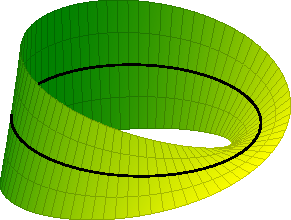
\includegraphics[width=0.5\linewidth, keepaspectratio]{figures/moebius-strip.pdf} 
    \caption{Möbiusband}
    \label{fig:moebius-strip}
\end{figure}

\section{Gauß-Krümmung}
\begin{bemerkung}\label{bem:18.1}%In Vorlesung: Bemerkung 18.1
    Sei $S$ eine reguläre Fläche, $s \in S$, $n(s)$ ist ein Normalenvektor
    in $s$, $x \in T_s (S)$, $\|x\| = 1$.

    Sei $E$ der von $x$ und $n(s)$ aufgespannte 2-dimensionale 
    Untervektorraum von $\mdr^3$.

    Dann gibt es eine Umgebung $V \subseteq \mdr^3$ von $s$, sodass
    \[C := (s + E) \cap S \cap V\]
    das Bild einer durch Bogenlänge parametrisierten Kurve
    $\gamma:[-\varepsilon, \varepsilon] \rightarrow s$ enthält mit
    $\gamma(0) = s$ und $\gamma'(0) = x$.
\end{bemerkung}

\begin{beweis}
    \enquote{Satz über implizite Funktionen}, siehe z.~B. 
    \href{https://github.com/MartinThoma/LaTeX-examples/tree/master/documents/Analysis\%20II}{\path{github.com/MartinThoma/LaTeX-examples/tree/master/documents/Analysis\%20II}}
\end{beweis}

\begin{definition}\xindex{Normalenkrümmung}%In Vorlesung: Definition 18.2
    In der Situation aus \cref{bem:18.1} heißt die Krümmung $\kappa_\gamma(0)$
    der Kurve $\gamma$ in der Ebene $(s+ E)$ im Punkt $s$ die
    \textbf{Normalenkrümmung}\footnotemark von $S$ in $s$ in Richtung
    $x = \gamma'(0)$.

    Man scheibt: $\kappa_\gamma(0) := \kappanor(s, x)$
\end{definition}
\footnotetext{Die Krümmung ist nur bis auf das Vorzeichen bestimmt.}

\begin{beispiel}%In Vorlesung: Beispiel 18.3
    \begin{bspenum}
        \item $S = S^2 = V(X^2 + Y^2 + Z^2 - 1)$ ist die Kugel um den Ursprung mit Radius~1,
              $n = \id$, $s=(0,0,1)$, $x=(1,0,0)$\\
              $\Rightarrow E = \mdr \cdot x + \mdr \cdot n(s)$ ($x,z\text{-Ebene}$)

              $C = E \cap S$ ist Kreislinie\\
              $\kappanor(s, x) = \frac{1}{r} = 1$
        \item $S = V(X^2 + Z^2 - 1) \subseteq \mdr^3$ ist ein Zylinder (siehe \cref{fig:regular-zylinder}).
              $s = (1,0,0)$\\
              $x_1 = (0,1,0) \Rightarrow E_1 = \mdr \cdot e_1 + \mdr \cdot e_2$ ($x,y\text{-Ebene}$)\\
              $S \cap E_1 = V(X^2 + Y^2 - 1) \cap E$, Kreislinie in $E$\\
              $\Rightarrow \kappanor(s, x_1) = \pm 1$\\
              $x_2 = (0, 0, 1), E_2 = \mdr \cdot e_1 + \mdr \cdot e_3$ ($x,z\text{-Ebene}$)\\
              $V \cap E_2 \cap S = \Set{(1, 0, z) \in \mdr^3 | z \in \mdr}$ ist eine Gerade\\
              $\Rightarrow \kappanor(s, x_2) = 0$
        \item $S = V(X^2 - Y^2 - Z)$, $s = (0,0,0)$ (Hyperbolisches Paraboloid\xindex{Paraboloid!hyperbolisches}, siehe \cref{fig:hyperbolic-paraboloid})\\
              $x_1 = (1,0,0)$, $n(s) = (0,0,1)$\\
              $x_2 = (0, 1, 0)$\\
              $\kappanor(s, x_1) = 2$\\
              $\kappanor(s, x_2) = -2$
    \end{bspenum}
\end{beispiel}

\begin{figure}[ht]
    \centering
    \subfloat[$S = V(X^2 + Z^2 - 1)$]{
        \resizebox{0.4\linewidth}{!}{\pgfplotsset{
    colormap={whitered}{
        color(0cm)=(white);
        color(1cm)=(orange!75!red)
    }
}
\begin{tikzpicture}
    \begin{axis}[
    colormap name=whitered,
    width=15cm,
    view={340}{25},
    enlargelimits=false,
    grid=major,
    domain=0:5,
    y domain=0:2*pi,
    xmin=-1.5, xmax=1.5,
    ymin=-1.5, ymax=1.5,  zmin=0.0,
    samples=30, %57 : TeX capacity exceeded, sorry [main memory size=3000000].
                % see also http://tex.stackexchange.com/a/7954/5645
    xlabel=$x$,
    ylabel=$y$,
    zlabel={$z$},
    %colorbar,
    colorbar style={
        at={(-0.1,0)},
        anchor=south west,
        height=0.25*\pgfkeysvalueof{/pgfplots/parent axis height},
        title={$f(x,y)$}
    }
    ]
    \addplot3 [surf,z buffer=sort] ({cos(deg(y))},{sin(deg(y))},{x});
    \end{axis}
\end{tikzpicture}
}
        \label{fig:regular-zylinder}
    }%
    \subfloat[$S = V(X^2 - Y^2 - Z)$]{
        \resizebox{0.4\linewidth}{!}{\documentclass[border=2pt]{standalone}
\usepackage{pgfplots}
\pgfplotsset{compat=1.9} %It is possible to remove this line, but you will get a warning

\begin{document}
\pgfplotsset{
    colormap={whitered}{
        color(0cm)=(white);
        color(1cm)=(orange!75!red)
    }
}
\begin{tikzpicture}
    \begin{axis}[
    colormap name=whitered,
    width=15cm,
    view={340}{25},
    enlargelimits=false,
    grid=major,
    domain=-2:2,
    y domain=-2:2,
    samples=40, %57 : TeX capacity exceeded, sorry [main memory size=3000000].
                % see also http://tex.stackexchange.com/a/7954/5645
    xlabel=$x$,
    ylabel=$y$,
    zlabel={$z$},
    colorbar,
    colorbar style={
        at={(-0.1,0)},
        anchor=south west,
        height=0.25*\pgfkeysvalueof{/pgfplots/parent axis height},
        title={$f(x,y)$}
    }
    ]
    \addplot3[surf,draw=black] {x^2-y^2};
    \end{axis}
\end{tikzpicture}
\end{document}
}
        \label{fig:hyperbolic-paraboloid}
    }%
    \label{fig:regular-surfaces}
    \caption{Beispiele für reguläre Flächen}
\end{figure}

%%%%%%%%%%%%%%%%%%%%%%%%%%%%%%%%%%%%%%%%%%%%%%%%%%%%%%%%%%%%%%%%%%%%%
% Mitschrieb vom 06.02.2014                                         %
%%%%%%%%%%%%%%%%%%%%%%%%%%%%%%%%%%%%%%%%%%%%%%%%%%%%%%%%%%%%%%%%%%%%%
\begin{definition}\xindex{Normalenkrümmung}%In Vorlesung: Def. 18.4
    Sei $S \in \mdr^3$ eine reguläre Fläche, $s \in S$, ($n$ ein
    stetiges Normalenfeld auf $S$)

    $\gamma:[-\varepsilon, \varepsilon] \rightarrow S$ eine nach
    Bogenlänge parametrisierte Kurve ($\varepsilon > 0$) mit
    $\gamma(0) = s$ und $\gamma''(0) \neq 0$.

    Sei $n(0) := \frac{\gamma''(0)}{\|\gamma''(0)\|}$. Zerlege
    $n(0) = n(0) + n(0)^\bot$ mit $n(0)^\bot \in T_s S$ und
    $n(0)^\bot \in (T_s S)^\bot$.

    Dann ist $n(0)^\bot = \langle n(0), n(s) \rangle \cdot n(s)$\\
    $\kappanor(s, \gamma) := \langle \gamma''(0), n(s) \rangle$
    die \textbf{Normalenkrümmung}.\todo{Ist das hier die Normalenkrümmung? Was ist mit der anderen Def.?}
\end{definition}

\begin{bemerkung}
    Sei $\overline{\gamma}(t) = \gamma(-t)$, $t \in [- \varepsilon, \varepsilon]$.
    Dann ist $\kappanor(s, \overline{\gamma}) = \kappanor(s, \gamma)$.
\end{bemerkung}

\begin{beweis}
    $\overline{\gamma}''(0) = \gamma''(0)$, da $\overline{\gamma}'(0) = - \gamma'(0)$.

    Es gilt: $\kappanor(s,\gamma)$ hängt nur von $|\gamma'(0)|$ ab
    und ist gleich $\kappanor(s, \gamma'(0))$.
\end{beweis}

\begin{bemerkung}%In Vorlesung: Bem.+Def. 18.6
    Sei $S$ eine reguläre Fläche und $n=n(s)$ ein Normalenvektor an 
    $S$ in $s$.

    Sei $T_{s}^{1} S = \Set{x \in T_s S | \|x\| = 1} \cong S^1$.
    Dann ist $\kappanor^n(s): T_s S \rightarrow \mdr$,
    $x \mapsto \kappanor(s,x)$ eine glatte Funktion und 
    $\Bild \kappanor(s)$ ist ein abgeschlossenes Intervall.
\end{bemerkung}

\begin{definition}\xindex{Hauptkrümmung}\xindex{Gauß-Krümmung}%In Vorlesung: Bem.+Def. 18.6
    Sei $S$ eine reguläre Fläche und $n=n(s)$ ein Normalenvektor an 
    $S$ in $s$.

    \begin{defenum}
        \item $\kappa^n_1(s) := \min \Set{\kappanor^n(s,x) | x \in T_s^1 S}$ und\\
              $\kappa^n_2(s) := \max \Set{\kappanor^n(s,x) | x \in T_s^1 S}$
              heißen \textbf{Hauptkrümmungen} von $S$ in $s$.
        \item $K(s) := \kappa_1^n(s) \cdot \kappa_2^n(s)$ heißt
              \textbf{Gauß-Krümmung} von $S$ in $s$.
    \end{defenum}
\end{definition}

\begin{bemerkung}%In Vorlesung: Bem.+Def. 18.6
    Ersetzt man $n$ durch $-n$, so gilt: $\kappanor^{-n}(s, x) = - \kappanor^n(x)\; \forall x \in T_s^1 S$\\
    $\Rightarrow \kappa_1^{-n}(s) = - \kappa_2^n(s)$,\\
    $\kappa_2^{-n}(s) = - \kappa_1^n (s)$\\
    und $K^{-n}(s) = K^n(s) =: K(s)$.
\end{bemerkung}

\begin{beispiel}
    \begin{bspenum}
        \item $S = S^2$. Dann ist $\kappa_1(s) = \kappa_2(s) = \pm 1\;\forall s \in S^2$\\
              $\Rightarrow K(s) = 1$
        \item Zylinder:\\
              $\kappa_1(s) = 0, \kappa_2(s) = 1 \Rightarrow K(s) = 0$
        \item Sattelpunkt auf hyperbolischem Paraboloid:\\
              $\kappa_1(s) < 0, \kappa_2(s) = 0 \rightarrow K(s) < 0$
        \item $S = \text{Torus}$. Siehe \cref{fig:torus-gauss-kruemmung}\\
            \begin{figure}[htp]\xindex{Torus}
                \centering
                % The following answers were used to create this image:
% - http://tex.stackexchange.com/a/373/5645 - Torus
\documentclass[border=2pt]{standalone}
\usepackage{amsmath,amssymb}
\usepackage{tikz}
\usetikzlibrary{patterns,arrows,positioning}

\begin{document}
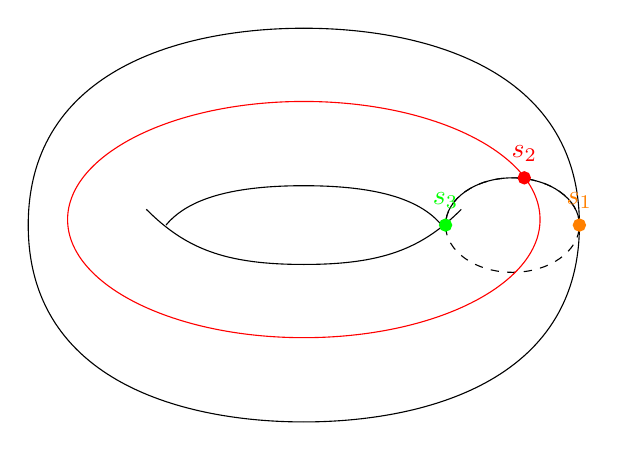
\begin{tikzpicture}
\tikzstyle{point}=[circle,thick,draw=black,fill=black,inner sep=0pt,minimum width=4pt,minimum height=4pt]
\draw (-3.5,0) .. controls (-3.5,2) and (-1.5,2.5) .. (0,2.5);
\draw[xscale=-1] (-3.5,0) .. controls (-3.5,2) and (-1.5,2.5) .. (0,2.5);
\draw[rotate=180] (-3.5,0) .. controls (-3.5,2) and (-1.5,2.5) .. (0,2.5);
\draw[yscale=-1] (-3.5,0) .. controls (-3.5,2) and (-1.5,2.5) .. (0,2.5);

\draw (-2,.2) .. controls (-1.5,-0.3) and (-1,-0.5) .. (0,-.5) .. controls (1,-0.5) and (1.5,-0.3) .. (2,0.2);
\draw (-1.75,0) .. controls (-1.5,0.3) and (-1,0.5) .. (0,.5) .. controls (1,0.5) and (1.5,0.3) .. (1.75,0);

\draw[dashed] (2.65,0) ellipse (0.85 and 0.6);
\draw (3.5,0) arc (-360:-180:0.85 and 0.6);

\node (s1)[point,orange,label={[label distance=0mm]\color{orange}$s_1$}] at (3.5,0) {};
\node (s2)[point,red,label={[label distance=0mm]\color{red}$s_2$}] at (2.8,0.6) {};
\node (s3)[point,green,label={[label distance=0mm]\color{green}$s_3$}] at (1.8,0) {};
\draw[red] (0,0.07) ellipse (3cm and 1.5cm);
\end{tikzpicture}
\end{document}
 
                \caption{$K(s_1) > 0$, $K(s_2) = 0$, $K(s_3) < 0$}
                \label{fig:torus-gauss-kruemmung}
            \end{figure}
    \end{bspenum}
\end{beispiel}

\begin{bemerkung}%In Vorlesung: Bem. 18.7
    Sei $S$ eine reguläre Fläche, $s \in S$ ein Punkt.
    \begin{bemenum}
        \item Ist $K(s) > 0$, so liegt $S$ in einer Umgebung von $s$
              ganz auf einer Seite von $T_s S + s$.
        \item Ist $K(s) < 0$, so schneidet jede Umgebung von $s$ in $S$
              beide Seiten von $T_s S + s$.
    \end{bemenum}
\end{bemerkung}

%%%%%%%%%%%%%%%%%%%%%%%%%%%%%%%%%%%%%%%%%%%%%%%%%%%%%%%%%%%%%%%%%%%%%
% Mitschrieb vom 11.02.2014                                         %
%%%%%%%%%%%%%%%%%%%%%%%%%%%%%%%%%%%%%%%%%%%%%%%%%%%%%%%%%%%%%%%%%%%%%
\section{Erste und zweite Fundamentalform}%In Vorlesung: §19
Sei $S \subseteq \mdr^3$ eine reguläre Fläche, $s \in S$, $T_s S$ die Tangentialebene
an $S$ in $s$.

\begin{bemerkung}%In Vorlesung: Bem.+Def. 19.1
    \begin{bemenum}
        \item \label{bem:19.1a} Die Einschränkung des Standardskalarproduktes des $\mdr^3$ auf
              $T_s S$ macht $T_s S$ zu einem euklidischen Vektorraum.
        \item Sei $F: U \rightarrow V$ eine lokale Parametrisierung von $S$ um
              $s$ und $p := F^{-1}(s)$.

              Dann ist $\Set{D_P F(e_1), D_P F(e_2)}$ eine Basis von $T_s S$.
        \item Bzgl. der Basis $\Set{D_P F(e_1), D_P F(e_2)}$ hat das 
              Standardskalarprodukt aus \cref{bem:19.1a} die Darstellungsmatrix
              \begin{align*}
                I_S &= \begin{pmatrix}
                          g_{1,1}(s) & g_{1,2}(s)\\
                          g_{1,2}(s) & g_{2,2}(s)
                       \end{pmatrix} =
                       \begin{pmatrix}
                          E(s) & F(s) \\
                          F(s) & G(s)
                       \end{pmatrix}\\
       \text{mit } g_{i,j} &= g_s(D_P F(e_i), D_P F(e_j))\\
                      &= \langle \frac{\partial F}{\partial u_i} (p), \frac{\partial F}{\partial u_j} (p) \rangle \;\;\; i,j \in \Set{1,2}
              \end{align*}
              Die Matrix $I_S$ heißt \textbf{erste Fundamentalform}\xindex{Fundamentalform!erste}
              von $S$ bzgl. der Parametrisierung $F$.
        \item $g_{i,j}(s)$ ist eine differenzierbare Funktion von $s$.
    \end{bemenum}
\end{bemerkung}

\begin{bemerkung}
    \[\det(I_S) = \left \| \frac{\partial F}{\partial u_1}(p) \times \frac{\partial F}{\partial u_2}(p) \right \|^2\] 
\end{bemerkung}

\begin{beweis}
    Sei $\frac{\partial F}{\partial u_1}(p) = \begin{pmatrix}
        x_1\\ x_2 \\ x_3
    \end{pmatrix}, \;\;\; \frac{\partial F}{\partial u_2}(p) = \begin{pmatrix}
        y_1\\ y_2 \\ y3
    \end{pmatrix}$

    Dann ist $\frac{\partial F}{\partial u_1}(p) \times \frac{\partial F}{\partial u_2}(p) = \begin{pmatrix}
        z_1 \\ z_2 \\ z_3
    \end{pmatrix}$ mit
    \begin{align*}
        z_1 &= x_2 y_3 - x_3 - y_2\\
        z_2 &= x_3 y_1 - x_1 y_3\\
        z_3 &= x_1 y_2 - x_2 y_1\\
    \Rightarrow \|\frac{\partial F}{\partial u_1} (p) \times \frac{\partial F}{\partial u_2} (p)\| &= z_1^2 + z_2^2 + z_3^2\\
    \end{align*}
    \begin{align*}
        \det(I_S) &= g_{1,1} g_{2,2} - g_{1,2}^2\\
        &= \left \langle \begin{pmatrix} x_1 \\ x_2 \\ x_3 \end{pmatrix}, \begin{pmatrix} x_1 \\ x_2 \\ x_3 \end{pmatrix} \right \rangle \left \langle \begin{pmatrix} y_1 \\ y_2 \\ y_3 \end{pmatrix}, \begin{pmatrix} y_1 \\ y_2 \\ y_3 \end{pmatrix} \right \rangle - \left \langle \begin{pmatrix} x_1 \\ x_2 \\ x_3 \end{pmatrix}, \begin{pmatrix} y_1 \\ y_2 \\ y_3 \end{pmatrix} \right \rangle^2\\
        &= (x_1^2 + x_2^2 + x_3^2) (y_1^2 + y_2^2 + y_3^2) - (x_1 y_1 + x_2 y_2 + x_3 y_3)^2
    \end{align*}
\end{beweis}

\begin{definition}\xindex{Flächenelement}%In Vorlesung: Def.+Bem. 19.3 / Erinnerung
    \begin{defenum}
        \item Das Differential
              \[\mathrm{d} A = \sqrt{\det (I)} \mathrm{d} u_1 \mathrm{d} u_2\]
              heißt \textbf{Flächenelement} von $S$ bzgl. der Parametrisierung $F$.
        \item \label{def:berechenbares-integral}Für eine Funktion $f: V \rightarrow \mdr$ heißt 
              \[\int_V f \mathrm{d} A := \int_U f(\underbrace{F(u_1, u_2)}_{=: s}) \sqrt{\det I(s)} \mathrm{d} u_1 \mathrm{d} u_2\]
              der \textbf{Wert des Integrals} von $f$ über $V$, falls das Integral rechts
              existiert.
    \end{defenum}

\end{definition}

\begin{bemerkung}
    \begin{bemenum}
        \item $\int_V f \mathrm{d} A$ ist unabhänig von der gewählten Parametrisierung.
        \item Sei $f: S \rightarrow \mdr$ eine Funktion, die im Sinne von
              \cref{def:berechenbares-integral} lokal integrierbar ist.

              Dann ist $\int_S f \mathrm{d} A$ wohldefiniert, falls (z.~B.) $S$
              kompakt ist.

              Etwa: $\int_S f \mathrm{d} A = \sum_{i=1}^n \int_{V_i} f \mathrm{d} A - \sum_{i \neq j} \int_{V_i \cap V_j} f \mathrm{d} A + \sum_{i,j,k} \int_{V_i \cap V_j \cap V_k} - \dots$
    \end{bemenum}
\end{bemerkung}

\begin{beweis}
    \begin{enumerate}[label=\alph*)]
        \item Mit Transformationsformel
        \item Ist dem Leser überlassen
    \end{enumerate}
\end{beweis}

\begin{proposition}
    Sei $S \subseteq \mdr^3$ eine reguläre, orientierbare Fläche mit glatten
    Normalenfeld $n: S \rightarrow S^2$.

    \begin{propenum}
        \item $n$ induziert für jedes $s \in S$ eine lineare Abbildung $d_S n: T_s S \rightarrow T_{n(s)} S^2$
              durch 
              \[d_s n(x) = \frac{\mathrm{d}}{\mathrm{d} t} n (\underbrace{s \text{\enquote{+}} tx}_{\mathclap{\text{Soll auf Fläche $S$ bleiben}}}) \Bigr |_{t=0}\]
        \item $T_{n(s)} S^2 = T_s S$
        \item $d_S n$ ist ein Endomorphismus von $T_s S$
        \item $d_S n$ ist selbstadjungiert bzgl. des Skalarproduktes $I_S$
    \end{propenum}
\end{proposition}

\begin{beweis}\leavevmode
    \begin{enumerate}[label=\alph*)]
        \item TODO
        \item $T_{n(S)} S^2 = \langle n(s) \rangle^\bot = T_s S$
        \item TODO
        \item Zu zeigen: $\forall x,y \in I_s S: \langle x, d_s n (y) \rangle = \langle d_s n(x), y \rangle$

        Aufgrund der Bilinearität des Skalarproduktes genügt es diese Eigenschaft
        für die Basisvektoren zu zeigen.

        Sei $x_i = D_P F(e_i) = \frac{\partial F}{\partial u_i} (p)\;\;\; i = 1,2$

        \underline{Beh.:} $\langle x_i, d_s n(x_j) \rangle = \langle \frac{\partial^2 F}{\partial u_i \partial u_j} (p), d_s n (x_i) \rangle$

        $\Rightarrow \langle \frac{\partial^2 F}{\partial u_i \partial u_j} (p), d_s n (x_i) \rangle = \langle x_j, d_s n (x_i) \rangle$

        \underline{Bew.:} 

        \begin{align*}
            0 &= \hphantom{\frac{\mathrm{d}}{\mathrm{d}t} \left (\right.} \langle \frac{\partial F}{\partial u} (p + t e_j), n(p + t e_j) \rangle\\
\Rightarrow 0 &= \frac{\mathrm{d}}{\mathrm{d}t} \left (\langle \frac{\partial F}{\partial u} (p + t e_j), n(p + t e_j) \rangle \right) \Bigr |_{t=0}\\
              &= \langle \underbrace{\frac{\mathrm{d}}{\mathrm{d}t} \frac{\partial F}{\partial u_i} (p + t e_j)}_{\frac{\partial^2 F}{\partial u_j \partial u_i} (p)} \Bigr |_{t=0}, n(s) \rangle + \langle x_i, d_s n \underbrace{D_P F (e_j)}_{x_j}\rangle
        \end{align*}
    \end{enumerate}
\end{beweis}